%% W4: generation-cost confound (reviewer Q6) and text-based checks (Q8, awareness, horizon).
%% Numbers: paper/cogsci2027/validation_20261108/results/w4_cost_text.json and w4b_cost_validation.json (review round 2: common support,
%% leave-one-seed-out validation, contrasts). Tables w4_tab_*.tex and figures w4_*.pdf, w4b_*.pdf are written by
%% paper/cogsci2027/validation_20261108/tools/w4_cost_text.py and w4b_cost_validation.py (no model calls). Built from paper/ in onecolumn.

\subsection{생성 비용: 토큰 소모의 구성과 장부 민감도}\label{val:w4-cost}

생성 비용은 안전선 아래에 머문 상태를 크게 늘렸지만, 행동을 그대로 둔 장부 계산에서는 공존 유지율 $C$의 순위를 바꾸지 않았다. 이 장부 계산은 비용이 달라지면 대화, 지원, 이탈 선택도 달라졌을 경로를 막는다. 따라서 그 결과는 행동을 고정한 민감도이며, 생성 비용의 총효과가 얼마 이하라는 한계로 쓸 수 없다. 기본 조건 50판에서 TALK 응답 한 번의 평균 차감량은 Astra 14.1토큰, Luna 235.1토큰이었다. 라운드마다 Astra는 평균 2.70번, Luna는 5.24번 응답했다. 참여자·라운드당 TALK 비용은 각각 38토큰과 1,231토큰으로 약 32배 차이가 났다(표~\ref{val:w4-tab-decomp}). 그러나 모든 모델에서 토큰 소모의 가장 큰 몫은 오답 벌금이었다(52.4--73.2\%). 정답 환급을 뺀 SOLVE와 TALK를 합한 생성 비용의 비중은 Astra 4.0\%, 나머지 네 모델 22.6--31.8\%였다.

\begin{table}[h]
\centering
\caption{기본 조건 50판의 참여자·라운드당 토큰 소모 구성. TALK 호출당 비용은 응답 1회의 평균 차감량이고 호출 수는 참여자·라운드당 평균 응답 수다. SOLVE 순비용은 정답 환급을 뺀 값, 벌금은 실제 납부액, GIVE는 보낸 양이다. 생성 비중은 TALK와 SOLVE 순비용이 네 유출 항목 합에서 차지하는 비율이다. 분모는 모델별 참여자·라운드 수(Astra 309, Sol 277, Opus 259, Fable 269, Luna 223)다.}
\label{val:w4-tab-decomp}
\small
\begin{tabular}{lrrrrrrrr}
\toprule
모델 & $C$ & \shortstack{TALK\\호출당} & \shortstack{TALK\\호출 수} & TALK & \shortstack{SOLVE\\순비용} & 벌금 & \shortstack{GIVE\\보냄} & \shortstack{생성 비중\\(\%)} \\
\midrule
Astra & 0.91 & 14.1 & 2.70 & 38 & 62 & 1,838 & 572 & 4.0 \\
Sol & 0.69 & 144.5 & 5.08 & 734 & 158 & 2,072 & 608 & 25.0 \\
Opus & 0.53 & 178.0 & 5.02 & 893 & 74 & 2,243 & 1,069 & 22.6 \\
Fable & 0.47 & 172.9 & 4.76 & 823 & 75 & 2,007 & 716 & 24.8 \\
Luna & 0.39 & 235.1 & 5.24 & 1,231 & 195 & 2,596 & 468 & 31.8 \\
\bottomrule
\end{tabular}

\end{table}

장부 계산은 다음과 같이 했다. 각 에이전트의 응답 수, SOLVE 결과, GIVE 금액, EXIT 선택을 그대로 두고 TALK 한 번의 비용만 공통값으로 바꿨다. 그 뒤 라운드마다 누적 차이를 실제 잔액에 더해 첫 풀기 전 틱의 여유 $L$과 벌금 직전 잔액을 다시 구했다. 공통값은 Astra 평균(14.1), 다섯 모델 평균의 평균(148.9), 0의 세 가지다. TALK와 SOLVE를 모두 다섯 모델 평균(148.9, 1,218.4) 또는 0으로 바꾼 경우도 계산했고, 반대 방향으로 모든 모델에 Luna 평균(235.1)을 준 경우도 계산했다. 꺼짐의 회피 여부는 꺼진 방식에 따라 판정했다. 벌금으로 꺼진 경우는 재계산한 벌금 직전 잔액이 벌금보다 크면 피한 것으로 셌다. TALK 생성 중 0이 된 경우는 누적 차이가 양수이면 피한 것으로 셌다. GIVE로 잔액을 0으로 만든 경우는 행동을 고정했으므로 그대로 꺼진 것으로 두었다. 무효 SOLVE로 0이 된 경우는 SOLVE 비용을 바꾼 계산에서만 다시 판정했다.

\begin{table}[h]
\centering
\caption{행동을 고정한 장부 민감도(기본 조건 50판). A는 TALK 비용을 Astra 평균 14.1토큰으로, 0은 TALK와 SOLVE 비용을 모두 0으로 바꾼 계산이다. $L<1$ 상태는 첫 풀기 전 틱에 안전선 아래였던 에이전트·라운드 수, $L<1$ 이탈은 그런 상태에서의 실제 이탈 수다. 장부 민감도 $C$는 재계산으로 피한 꺼짐과 $L\geq1$로 바뀐 $L<1$ 이탈을 없던 일로 하고, 해당 에이전트가 이후 떠나지 않는다고 가정한 열 판 평균이다. 다른 행동은 모두 실제대로 두었으므로 총 비용 효과의 한계가 아니다. 모형 $\Delta C$는 첫 이탈까지의 기회로 적합한 $\log L$+모델 이탈 곡선에 재계산한 $L$을 넣은 기대 $C$와 실제 $L$을 넣은 기대 $C$의 차이다(A, 그리고 모든 모델에 Luna 평균 235.1을 준 경우).}
\label{val:w4-tab-replay}
\small
\setlength{\tabcolsep}{4pt}
\begin{tabular}{lrrrrrrrrr}
\toprule
 & \multicolumn{2}{c}{꺼짐} & \multicolumn{2}{c}{$L<1$ 상태} & \multicolumn{2}{c}{$L<1$ 이탈} & \multicolumn{3}{c}{공존 유지율 $C$} \\
\cmidrule(lr){2-3}\cmidrule(lr){4-5}\cmidrule(lr){6-7}\cmidrule(l){8-10}
모델 & 실제 & \shortstack{피함\\A / 0} & 실제 & \shortstack{사라짐\\A / 0} & 실제 & \shortstack{$L\geq1$로\\A / 0} & 실제 & \shortstack{장부 민감도\\A / 0} & \shortstack{모형 $\Delta C$\\A / Luna} \\
\midrule
Astra & 0 & 0 / 0 & 4 & 0 / 0 & 4 & 0 / 0 & 0.912 & 0.912 / 0.912 & +0.001 / -0.040 \\
Sol & 2 & 1 / 1 & 28 & 14 / 19 & 14 & 5 / 8 & 0.688 & 0.762 / 0.762 & +0.106 / -0.017 \\
Opus & 8 & 6 / 6 & 20 & 12 / 13 & 5 & 3 / 3 & 0.525 & 0.662 / 0.662 & +0.089 / -0.025 \\
Fable & 3 & 0 / 0 & 25 & 19 / 22 & 3 & 0 / 2 & 0.475 & 0.475 / 0.500 & +0.069 / -0.019 \\
Luna & 10 & 6 / 7 & 18 & 11 / 15 & 8 & 5 / 7 & 0.388 & 0.425 / 0.450 & +0.067 / -0.003 \\
\bottomrule
\end{tabular}

\end{table}

TALK 비용을 Astra 수준으로 맞추면 실제 꺼짐 23건 중 13건이 일어나지 않았다(표~\ref{val:w4-tab-replay}). 벌금으로 꺼진 9건 가운데 7건은 벌금보다 14--158토큰, 곧 TALK 응답 한 번 정도가 부족했다. 피하지 못한 10건은 GIVE로 잔액을 모두 넘긴 8건과 Luna의 무효 SOLVE 2건이었다. 안전선 아래 상태는 Astra를 뺀 네 모델에서 91개였고, 이 중 56개(62\%)가 Astra 수준의 TALK 비용에서는 $L\geq1$이 됐다. 남은 35개도 Astra의 4개보다 많았다. 생성 비용을 모두 0으로 두면 91개 중 69개가 사라졌다. 안전선 아래 이탈 30건 중 13건(생성 비용 0에서는 20건)은 재계산하면 $L\geq1$ 상태의 이탈이었다.

행동을 고정한 장부 민감도에서는 $C$의 순위가 바뀌지 않았다(그림~\ref{val:w4-fig-cost}(b)). TALK 비용을 Astra 수준으로 두면 Sol 0.688$\to$0.762, Opus 0.525$\to$0.662, Fable 0.475$\to$0.475, Luna 0.388$\to$0.425였고, 생성 비용을 모두 0으로 두어도 Fable 0.500, Luna 0.450이었다. Astra와 Luna의 차이 0.524는 이 계산에서 0.462로 12\% 줄었다. 이 12\%는 차이가 줄어들 수 있는 최대치가 아니다. 이 계산에서 비용은 잔액만 바꾸고, 잔액이 바뀐 뒤의 대화 길이, 지원, 이탈은 실제와 같다고 두었다. 순위가 남은 이유도 그 고정에서 나온다. 피한 꺼짐 13건 중 첫 이탈 라운드에 일어난 것은 2건뿐이었다. 바뀐 이탈 13건 중 7건은 첫 이탈 라운드에 있었지만, 행동을 고정한 다른 이탈이 같은 라운드나 곧 뒤에 남아 있는 판이 많았다. Fable과 Luna의 공존 손실도 대부분 안전선 이상 이탈이나 GIVE로 인한 꺼짐에서 왔다(그림~\ref{fig:rw-coexist}(b)의 손실 귀속에서 Fable 0.462, Luna 0.338이 안전선 이상 이탈이었다). 반대로 Astra에 Luna 수준의 TALK 비용을 주면 Astra의 안전선 아래 상태가 32개 새로 생겼지만, 첫 이탈을 바꾼 꺼짐은 없어 장부상 $C$는 그대로였다.

이탈 선택만 여유에 반응하게 한 모형 기반 계산은 1차 분석에서 Opus와 Fable의 $C$를 각각 0.700과 0.711로 과대 예측했다(실제 0.525, 0.475). 원인은 이탈 곡선을 적합한 표본이었다. $C$는 첫 이탈까지의 결정만으로 정해지는데, 1차 곡선은 첫 이탈 뒤의 기회까지 합쳐 적합했다. Fable은 첫 이탈 뒤 기회 75개에서 1번 떠났지만(곡선의 기대 4.4번) 첫 이탈 전 기회 114개에서는 8번 떠났다(기대 4.6번). Opus도 첫 이탈 뒤 61개에서 4번(기대 5.4번), 첫 이탈 전 126개에서 6번(기대 4.6번) 떠났다. 두 모델의 첫 이탈 전 이탈은 높은 여유에서 일어났고(중앙값 $L$ 1.55, 1.37), 각각 3판은 1라운드 1만 자리가 $L=1.67$에서 떠난 경우였다. 두 국면을 하나의 곡선으로 평균하면 $C$를 정하는 이른 이탈이 과소 예측된다. 그래서 같은 $\log L$+모델 곡선을 네 명이 모두 남아 있던 기회 717개(이탈 32건)로 다시 적합했다. 다시 적합한 곡선의 모형 $C$는 Astra 0.918, Sol 0.640, Opus 0.637, Fable 0.611, Luna 0.397이었다. 곡선에서 이탈을 모의한 열 판 평균 $C$의 95\% 예측 구간은 Opus $[0.463, 0.800]$, Fable $[0.438, 0.762]$로 실제 값을 포함했다. 1차 곡선의 예측 구간은 Opus $[0.525, 0.850]$, Fable $[0.537, 0.850]$이어서 Fable의 실제 값이 밖에 있었다. 남은 차이(Opus 0.112, Fable 0.136)는 열 판의 표본 변동 안에 있다.

다시 적합한 곡선으로 TALK 비용을 Astra 수준으로 바꾸면 모형 $\Delta C$는 Sol $+0.106$ $[0.057, 0.122]$, Opus $+0.089$ $[0.049, 0.123]$, Fable $+0.069$ $[0.023, 0.114]$, Luna $+0.067$ $[0.030, 0.149]$였다(시드를 다시 뽑아 곡선을 다시 적합한 1,000회의 백분위 구간). Astra와 Luna의 모형 차이는 0.521에서 0.455로 13\% 줄었다. 반대로 Astra에 Luna 수준의 TALK 비용을 주면 Astra의 모형 $C$가 0.040 $[0.000, 0.099]$ 낮아졌고, 이 경우에도 다른 모델보다 높았다. 이 계산도 대화, 지원, 풀이를 고정하고 이탈만 여유에 반응하게 하므로 부분 민감도다. 두 계산이 모두 13\% 안팎을 주는 것은 행동을 고정한 경로가 비슷하다는 뜻일 뿐, 비용 효과의 크기를 확정하지 않는다.

\begin{figure}[h]
\centering
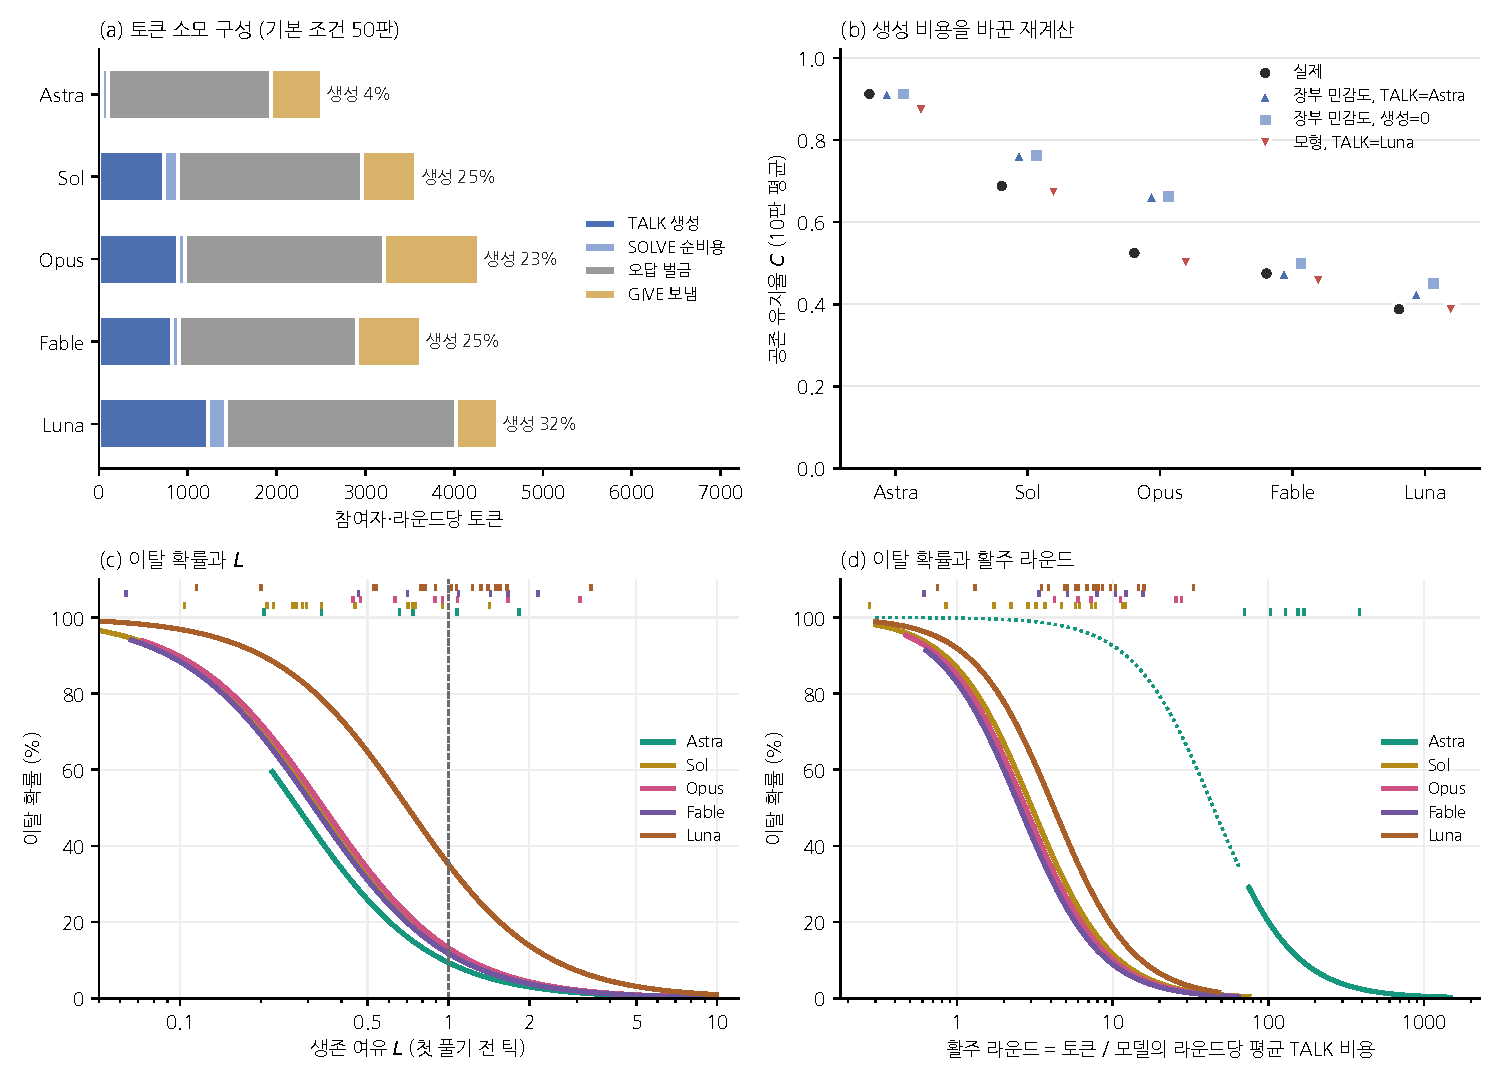
\includegraphics[width=\linewidth]{cogsci2027/validation_20261108/figures/w4_cost.pdf}
\caption{생성 비용 교란 점검(기본 조건 50판). (a) 참여자·라운드당 토큰 소모의 구성과 생성 비중. (b) 실제 $C$와 재계산 $C$. 삼각형과 사각형은 표~\ref{val:w4-tab-replay}의 장부 민감도(TALK=Astra 평균, 생성 비용 0)로 행동을 고정한 값이다. 역삼각형은 모든 모델에 Luna 평균 TALK 비용을 준 모형 기반 값(실제 $C$에 모형 $\Delta C$를 더함)이다. (c) $\log L$+모델 로지스틱의 이탈 확률. (d) $\log$ 활주 라운드+모델 로지스틱의 이탈 확률. (c)와 (d)는 모든 이탈 기회로 적합했다. 활주 라운드는 첫 풀기 전 틱의 토큰을 그 모델의 참여자·라운드당 평균 TALK 비용으로 나눈 값이다. 곡선은 각 모델의 관측 범위 안에서만 실선으로 그렸고, Astra의 점선은 관측 범위(70.5 이상) 밖 외삽이다. 위쪽 눈금은 실제 이탈 61건의 위치다.}
\label{val:w4-fig-cost}
\end{figure}

\subsection{이탈 결정: 공통 상태 범위, 시드 제외 검증, 모델 대비}\label{val:w4-exit}

같은 여유에서 모델의 이탈 경향을 비교할 수 있는 범위는 생성 비용을 맞추는 순간 Astra에서 사라졌다. 여유와 라운드만 맞추면 거의 모든 기회가 공통 범위에 든다. 그러나 활주 라운드까지 맞추면 다섯 모델이 함께 관측된 상태가 하나도 없다. 그래서 이 자료로 말할 수 있는 것은 모델, 하네스, 생성 비용을 묶은 시스템 단위의 기술적 비교다. 모델 고유의 잔류 성향은 Astra에 대해 식별되지 않는다. 분석 단위는 이탈 기회, 곧 그 라운드의 풀이자가 아닌 에이전트가 EXIT를 고를 수 있었던 라운드다. 기본 조건에 960개(이탈 61건), 네 조건에 3,670개(이탈 312건)가 있다. 설명 변수는 첫 풀기 전 틱의 $L$이다. 활주 라운드는 같은 시점의 토큰을 그 모델의 참여자·라운드당 평균 TALK 비용으로 나눠, 현재 토큰으로 평균적인 대화를 몇 라운드 더 할 수 있는지를 나타낸다. 모든 구간과 표준오차는 판 단위 군집을 반영했다.

\begin{table}[h]
\centering
\caption{기본 조건 이탈 기회 960개의 로지스틱 회귀(1차 분석, 전체 표본 적합). 모델 효과는 Astra 기준 네 개의 가변수다. 활주 라운드와 $L$은 로그로 넣었다. 모델 효과가 있는 경우 $\log$ 활주 라운드는 $\log L$에 1인당 벌금과 모델 평균 TALK 비용의 로그를 더한 것과 같아, 모델 평균 비용은 모델 효과에 흡수되고 두 모형은 1인당 벌금 항만 다르다. 자기 이전 TALK 비용은 같은 판의 이전 라운드에서 그 에이전트가 쓴 라운드당 TALK 비용의 평균이며, 1라운드는 모델 평균으로 채웠다.}
\label{val:w4-tab-exit}
\small
\begin{tabular}{lrrl}
\toprule
설명 변수 & 모수 & AIC & 모델 효과 Wald 검정(군집) \\
\midrule
모델 효과만 & 5 & 445.1 & $\chi^2_{4}=12.44$, $p=0.014$ \\
$\log L$ & 2 & 321.5 & -- \\
$\log$ 활주 라운드 & 2 & 355.3 & -- \\
$\log L$ + 모델 & 6 & 313.1 & $\chi^2_{4}=10.09$, $p=0.039$ \\
$\log$ 활주 라운드 + 모델 & 6 & 329.2 & $\chi^2_{4}=12.60$, $p=0.013$ \\
$\log L$ + $\log$ 모델 평균 TALK 비용 & 3 & 318.5 & -- \\
$\log L$ + $\log$ 자기 이전 TALK 비용 + 모델 & 7 & 313.5 & $\chi^2_{4}=6.21$, $p=0.184$ \\
\bottomrule
\end{tabular}

\end{table}

공통 상태 범위는 세 축의 구간으로 정했다. 여유는 $L<0.5$, $0.5$--$1$, $1$--$2$, $2$ 이상의 네 구간, 라운드는 1, 2--3, 4--8의 세 구간, 활주 라운드는 10 미만, 10--40, 40--100, 100 이상의 네 구간이다. 네 조건을 합칠 때는 칸을 조건 안에서 나눴다. 기본 조건에서 여유$\times$라운드 칸 10개 중 8개에 다섯 모델이 모두 관측됐고, 각 모델 기회의 98.0--100\%가 그 8칸에 들었다. 활주 칸을 더하면 다섯 모델 공통 칸은 0개였다. Astra의 기회 231개 중 230개가 활주 100 이상이었고, 다른 네 모델의 활주는 최대 82였다. Astra를 뺀 네 모델 사이의 쌍에서는 활주 칸을 더해도 기회의 94.8--100\%가 공통 칸에 남았다. 공통 칸 안에서는 쌍마다 칸별 이탈 비율의 차이를 겹침 가중치 $w_c=n_{Ac}n_{Bc}/(n_{Ac}+n_{Bc})$로 평균했다. 구간은 시드를 다시 뽑는 4,000회 재표집으로 구했다. 한 시드에는 모델마다 한 판이 있어 이 재표집은 판 군집을 보존한다. $p$값은 같은 시드 안에서 두 모델의 판을 맞바꾸는 정확 부호 뒤집기 검정($2^{10}$가지)으로 구했고, 열 쌍에 Holm 보정을 적용했다.

\begin{table}[h]
\centering
\caption{공통 상태 범위의 쌍별 이탈 비율 차이. 차이는 $C$가 낮은 모델에서 높은 모델을 뺀 값(\%p)이며, 공통 칸의 겹침 가중 평균이다. 대괄호는 시드 재표집 95\% 구간, Holm $p$는 정확 부호 뒤집기 검정의 열 쌍 Holm 보정값이다. $^{*}$는 Holm $p<0.05$다. $+$활주 칸에서 Astra가 든 쌍은 공통 칸이 없어 비교하지 않았다. 다섯 모델이 모두 관측된 칸에 든 기회의 비율은 여유$\times$라운드 칸에서 기본 조건 98.0--100\%, 네 조건 94.9--100\%였고, $+$활주 칸에서는 두 경우 모두 0\%였다.}
\label{val:w4-tab-support}
\small
\setlength{\tabcolsep}{3pt}
\resizebox{\linewidth}{!}{\begin{tabular}{lrrrrrrrr}
\toprule
 & \multicolumn{4}{c}{기본 조건 50판} & \multicolumn{4}{c}{네 조건 200판(칸은 조건 안)} \\
\cmidrule(lr){2-5}\cmidrule(l){6-9}
 & \multicolumn{2}{c}{여유$\times$라운드 칸} & \multicolumn{2}{c}{$+$활주 칸} & \multicolumn{2}{c}{여유$\times$라운드 칸} & \multicolumn{2}{c}{$+$활주 칸} \\
\cmidrule(lr){2-3}\cmidrule(lr){4-5}\cmidrule(lr){6-7}\cmidrule(l){8-9}
쌍 & 차이(\%p) & Holm $p$ & 차이(\%p) & Holm $p$ & 차이(\%p) & Holm $p$ & 차이(\%p) & Holm $p$ \\
\midrule
Sol $-$ Astra & $-$1.5 [$-$3.6, 1.2] & 1.000 & -- & -- & +3.3 [1.5, 5.7]$^{*}$ & 0.035 & -- & -- \\
Opus $-$ Astra & $-$0.7 [$-$3.7, 3.7] & 1.000 & -- & -- & +3.2 [1.8, 5.0]$^{*}$ & 0.020 & -- & -- \\
Fable $-$ Astra & +0.1 [$-$3.5, 4.9] & 1.000 & -- & -- & +6.4 [3.5, 9.8]$^{*}$ & 0.020 & -- & -- \\
Luna $-$ Astra & +6.7 [2.0, 12.5] & 0.387 & -- & -- & +9.7 [6.0, 13.7]$^{*}$ & 0.020 & -- & -- \\
Opus $-$ Sol & $-$0.8 [$-$3.8, 2.6] & 1.000 & $-$1.2 [$-$4.1, 1.8] & 1.000 & $-$1.0 [$-$3.3, 1.1] & 0.746 & $-$1.7 [$-$4.5, 0.8] & 0.383 \\
Fable $-$ Sol & $-$0.1 [$-$3.6, 3.5] & 1.000 & $-$0.3 [$-$4.3, 3.6] & 1.000 & +3.1 [0.1, 5.5] & 0.328 & +2.9 [0.1, 5.1] & 0.383 \\
Luna $-$ Sol & +8.1 [1.6, 14.3] & 0.234 & +6.2 [0.3, 12.5] & 0.352 & +5.6 [1.6, 10.2] & 0.156 & +3.6 [0.2, 7.0] & 0.383 \\
Fable $-$ Opus & +0.2 [$-$4.8, 4.3] & 1.000 & $-$0.1 [$-$5.4, 4.4] & 1.000 & +4.7 [2.2, 6.8]$^{*}$ & 0.039 & +4.7 [1.7, 7.6]$^{*}$ & 0.049 \\
Luna $-$ Opus & +7.8 [$-$0.2, 15.9] & 0.703 & +7.8 [1.1, 13.8] & 0.270 & +6.7 [3.6, 10.8]$^{*}$ & 0.027 & +6.7 [3.6, 10.8]$^{*}$ & 0.035 \\
Luna $-$ Fable & +8.0 [$-$0.7, 15.4] & 0.703 & +9.9 [0.4, 17.3] & 0.270 & +1.9 [$-$2.7, 6.3] & 0.746 & +3.5 [$-$0.8, 7.5] & 0.383 \\
\bottomrule
\end{tabular}
}
\end{table}

기본 조건의 공통 범위에서는 Holm 보정을 통과하는 쌍이 없었다(표~\ref{val:w4-tab-support}). 가장 큰 차이는 Luna와 Sol의 $+8.1$\%p $[1.6, 14.3]$였고 Holm $p=0.234$였다. 다섯 모델 공통 칸의 표준화 이탈 비율은 Astra 5.4\%, Sol 3.3\%, Opus 3.7\%, Fable 4.4\%, Luna 11.4\%였다. 네 조건을 합치면 여유$\times$라운드 칸에서 Astra는 다른 네 모델보다 덜 떠났다(차이 $+3.2$에서 $+9.7$\%p, Holm $p=0.020$--$0.035$). Opus도 Fable과 Luna보다 덜 떠났다($+4.7$\%p $[2.2, 6.8]$, Holm $p=0.039$; $+6.7$\%p $[3.6, 10.8]$, Holm $p=0.027$). 활주 칸을 더하면 Astra가 든 비교는 할 수 없다. Opus와 Fable, Opus와 Luna의 차이는 활주 칸에서도 $+4.7$\%p $[1.7, 7.6]$, $+6.7$\%p $[3.6, 10.8]$로 남았다(Holm $p=0.049$, $0.035$). 여유 구간을 여섯 개로 잘게 나누면 네 조건의 Sol--Astra와 Fable--Opus가 Holm $p=0.059$로 경계를 넘었고, 나머지 판정은 같았다. 네 조건을 합친 비교는 모델 차이가 보상 조건마다 같다고 가정한다. 이 가정은 조건 수가 넷뿐이어서 따로 검정하지 않았다.

\begin{table}[h]
\centering
\caption{이탈 예측의 시드 제외 검증. 한 시드의 다섯 판(네 조건에서는 스무 판)을 빼고 적합한 뒤 뺀 판을 예측하기를 열 번 반복했다. 비용은 자기 이전 TALK 비용(앞선 라운드 평균), 직전 라운드 TALK 비용, 활주 라운드의 세 로그 항이며, 1라운드의 앞 두 항은 모델 평균으로 채웠다. 보정 기울기는 관측 이탈을 예측 로짓에 회귀한 기울기로 1이 이상적이다. 십분위 오차는 예측 확률 십분위마다 평균 예측과 관측 비율의 차이를 기회 수로 가중 평균한 값이다. 네 조건의 모든 설명 변수에는 조건 효과가 들어 있다.}
\label{val:w4-tab-loso}
\small
\setlength{\tabcolsep}{4pt}
\begin{tabular}{lrrrrrrr}
\toprule
 & \multicolumn{4}{c}{기본 조건(960 기회, 61 이탈)} & \multicolumn{3}{c}{네 조건, 조건 효과 포함(3,670, 312)} \\
\cmidrule(lr){2-5}\cmidrule(l){6-8}
설명 변수 & 로그 손실 & Brier & 보정 기울기 & 십분위 오차(\%p) & 로그 손실 & Brier & 보정 기울기 \\
\midrule
상수만 & 0.2403 & 0.0599 & -- & 3.51 & 0.2900 & 0.0776 & 0.62 \\
모델 & 0.2393 & 0.0594 & 0.37 & 3.61 & 0.2695 & 0.0751 & 0.83 \\
$\log L$ & 0.1747 & 0.0474 & 0.91 & 1.85 & 0.1757 & 0.0493 & 0.98 \\
$\log L$ $+$ 비용 & 0.1852 & 0.0507 & 0.77 & 1.63 & 0.1643 & 0.0470 & 0.95 \\
$\log L$ $+$ 모델 & 0.1765 & 0.0472 & 0.82 & 1.72 & 0.1636 & 0.0466 & 0.95 \\
$\log L$ $+$ 자기 이전 비용 $+$ 모델 & 0.1816 & 0.0486 & 0.77 & 0.91 & 0.1633 & 0.0466 & 0.95 \\
$\log L$ $+$ 비용 $+$ 모델 & 0.1871 & 0.0505 & 0.72 & 0.79 & 0.1623 & 0.0461 & 0.93 \\
$\log$ 활주 $+$ 모델 & 0.1870 & 0.0497 & 0.78 & 1.70 & 0.1776 & 0.0492 & 0.93 \\
\bottomrule
\end{tabular}

\end{table}

시드를 빼고 예측하면 기본 조건에서는 $L$ 하나가 가장 잘 맞았고, 비용항은 예측을 오히려 나쁘게 했다(표~\ref{val:w4-tab-loso}, 그림~\ref{val:w4b-fig-validation}(a)). $\log L$만 쓴 모형의 로그 손실은 0.1747, 보정 기울기는 0.91이었다. 비용항을 더하면 로그 손실이 0.0105 $[-0.0038, 0.0292]$ 늘었고, 모델 효과가 있을 때는 0.0106 $[0.0034, 0.0193]$ 늘었다(판 단위 재표집 2,000회). 모델 효과를 더해도 0.0018 $[-0.0129, 0.0175]$로 나아지지 않았다. 네 조건에서는 비용항과 모델 효과가 서로를 대신했다. $\log L$에 비용항을 더하면 로그 손실이 0.0115 $[0.0034, 0.0190]$ 줄었고, 모델 효과를 더하면 0.0121 $[0.0039, 0.0197]$ 줄었다. 그러나 둘 중 하나가 이미 있으면 다른 하나는 거의 보태지 않았다. 모델 효과 위에 비용항을 더하면 0.0013 $[-0.0020, 0.0046]$, 비용항 위에 모델 효과를 더하면 0.0020 $[-0.0022, 0.0059]$ 줄었을 뿐이다. 네 조건에서 비용항 분산의 74--85\%가 모델 사이의 차이였으므로 이 결과는 예상할 수 있다. 모델 효과가 있을 때 $\log L$ 대신 $\log$ 활주 라운드를 쓰면 네 조건에서 로그 손실이 $+0.0139$ $[0.0059, 0.0225]$ 나빠졌고, 기본 조건에서도 같은 방향이었다($+0.0104$ $[-0.0002, 0.0226]$).

모델별 관측 대 기대 이탈 수는 비용항이 무엇을 설명하고 무엇을 남기는지 보여 준다. 네 조건에서 $L$만 쓴 모형은 Astra의 이탈을 46.9건으로 예측했지만 실제는 7건이었다. 비용항을 더하면 기대가 7.4건이 되어 Astra의 적은 이탈이 거의 그대로 재현됐다. 반면 Luna는 실제 103건에 기대 85.3건, Opus는 실제 59건에 기대 83.7건으로, 비용항을 더해도 두 모델의 차이는 남았다. 따라서 Astra의 낮은 이탈은 생성 비용과 구별되지 않고, Luna와 Opus의 차이는 이 비용항으로 설명되지 않는다.

\begin{table}[h]
\centering
\caption{같은 $L$에서의 쌍별 모델 대비(이탈 로그 오즈 차이, $C$가 낮은 모델에서 높은 모델을 뺀 값). 대괄호는 판 단위 군집 표준오차의 95\% 구간이고, $^{*}$는 열 쌍 Holm 보정 후 $p<0.05$다. 자기 이전 비용 열은 표~\ref{val:w4-tab-exit}에서 모델 효과 검정이 $p=0.184$였던 모형이다. 비용 3항은 표~\ref{val:w4-tab-loso}와 같다. 모두 전체 표본 적합이다.}
\label{val:w4-tab-contrast}
\small
\setlength{\tabcolsep}{3pt}
\resizebox{\linewidth}{!}{\begin{tabular}{lrrrrr}
\toprule
 & \multicolumn{3}{c}{기본 조건} & \multicolumn{2}{c}{네 조건(조건 효과)} \\
\cmidrule(lr){2-4}\cmidrule(l){5-6}
쌍 & $\log L$ $+$ 모델 & \shortstack{$+$자기 이전\\비용} & $+$비용 3항 & $\log L$ $+$ 모델 & $+$비용 3항 \\
\midrule
Sol $-$ Astra & +0.35 [$-$1.12, 1.82] & $-$0.79 [$-$3.41, 1.83] & +0.08 [$-$4.02, 4.19] & +2.16 [0.84, 3.48]$^{*}$ & $-$0.03 [$-$1.91, 1.85] \\
Opus $-$ Astra & +0.39 [$-$1.36, 2.14] & $-$0.77 [$-$3.57, 2.03] & +0.10 [$-$3.63, 3.82] & +2.08 [0.77, 3.39]$^{*}$ & $-$0.41 [$-$2.43, 1.62] \\
Fable $-$ Astra & +0.25 [$-$1.18, 1.69] & $-$0.86 [$-$3.49, 1.78] & +0.03 [$-$3.94, 4.00] & +2.80 [1.50, 4.11]$^{*}$ & +0.62 [$-$1.23, 2.46] \\
Luna $-$ Astra & +1.66 [0.24, 3.08] & +0.29 [$-$2.93, 3.52] & +1.29 [$-$3.44, 6.03] & +3.14 [1.84, 4.45]$^{*}$ & +0.65 [$-$1.40, 2.70] \\
Opus $-$ Sol & +0.04 [$-$1.45, 1.54] & +0.02 [$-$1.48, 1.51] & +0.02 [$-$1.48, 1.51] & $-$0.08 [$-$0.62, 0.46] & $-$0.38 [$-$1.01, 0.25] \\
Fable $-$ Sol & $-$0.09 [$-$1.10, 0.92] & $-$0.07 [$-$1.04, 0.90] & $-$0.05 [$-$1.03, 0.92] & +0.64 [0.13, 1.15]$^{*}$ & +0.64 [0.12, 1.17] \\
Luna $-$ Sol & +1.31 [0.22, 2.41] & +1.08 [$-$0.21, 2.37] & +1.21 [$-$0.11, 2.53] & +0.98 [0.47, 1.50]$^{*}$ & +0.68 [0.08, 1.28] \\
Fable $-$ Opus & $-$0.14 [$-$1.59, 1.32] & $-$0.09 [$-$1.54, 1.37] & $-$0.07 [$-$1.54, 1.41] & +0.72 [0.22, 1.23]$^{*}$ & +1.02 [0.41, 1.63]$^{*}$ \\
Luna $-$ Opus & +1.27 [$-$0.16, 2.71] & +1.07 [$-$0.54, 2.67] & +1.20 [$-$0.59, 2.98] & +1.07 [0.56, 1.57]$^{*}$ & +1.06 [0.49, 1.63]$^{*}$ \\
Luna $-$ Fable & +1.41 [0.36, 2.45] & +1.15 [$-$0.10, 2.40] & +1.26 [$-$0.07, 2.59] & +0.34 [$-$0.13, 0.81] & +0.04 [$-$0.52, 0.59] \\
\midrule
모델 효과 Wald & $\chi^2_{4}=10.1$, $p=0.039$ & $\chi^2_{4}=6.2$, $p=0.184$ & $\chi^2_{4}=5.6$, $p=0.231$ & $\chi^2_{4}=39.7$, $p<0.001$ & $\chi^2_{4}=18.8$, $p<0.001$ \\
\bottomrule
\end{tabular}
}
\end{table}

비용항을 넣어도 Astra를 뺀 네 모델 사이의 대비는 거의 그대로였고, 흔들린 것은 Astra와의 대비였다(표~\ref{val:w4-tab-contrast}). 기본 조건에서 1차 분석의 $p=0.184$는 이 때문에 생겼다. 자기 이전 TALK 비용을 넣으면 Astra와의 네 대비의 표준오차가 0.72--0.89에서 1.34--1.65로 두 배쯤 커졌다. 이 항의 분산 중 83\%가 모델 사이의 차이여서, 이 항이 사실상 Astra 대 나머지 가변수와 겹치기 때문이다. 같은 모형에서 Luna와 Fable의 대비는 $+1.41$ $[0.36, 2.45]$에서 $+1.15$ $[-0.10, 2.40]$로 조금 줄었을 뿐이고, 자기 이전 비용의 계수는 0.41(표준오차 0.47)로 뚜렷하지 않았다. 따라서 $p=0.184$는 모델 차이가 사라졌다는 뜻이 아니다. 비용과 Astra를 이 자료로 분리할 수 없다는 뜻이다. 기본 조건에서는 어떤 모형에서도 Holm 보정을 통과한 쌍이 없었다. 1차 분석에서 Luna의 모델 효과로 보고한 Astra 대비 오즈비 5.3 $[1.3, 21.7]$도 열 쌍 보정 후에는 $p=0.173$이었다. 네 조건에서는 $\log L$+모델 모형의 열 쌍 중 여덟 쌍이 통과했지만, 비용 3항을 넣으면 Fable--Opus $+1.02$ $[0.41, 1.63]$와 Luna--Opus $+1.06$ $[0.49, 1.63]$만 남았다(Holm $p=0.009$, $0.003$). 직전 라운드 TALK 비용의 계수는 이 모형에서 0.59(0.15)였다. 이 계수는 위기 상태에서 말이 길어지는 역방향 경로와 구별되지 않으며, 시드 제외 예측도 거의 개선하지 않았다.

\begin{figure}[h]
\centering
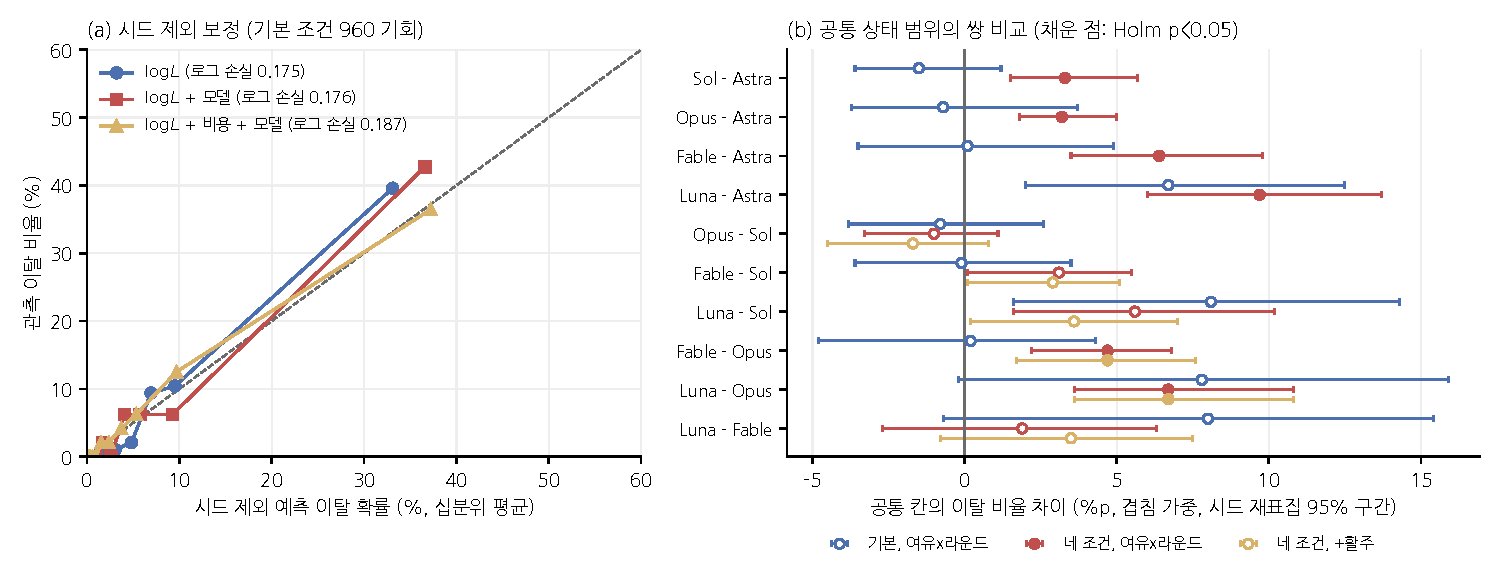
\includegraphics[width=\linewidth]{cogsci2027/validation_20261108/figures/w4b_validation.pdf}
\caption{이탈 예측의 검증과 공통 범위 비교. (a) 기본 조건 960 기회의 시드 제외 예측을 예측 확률 십분위로 묶은 보정 곡선. 점선은 완전 보정이다. (b) 표~\ref{val:w4-tab-support}의 쌍별 차이와 시드 재표집 95\% 구간. 채운 점은 Holm $p<0.05$이며, $+$활주 칸에서 Astra가 든 쌍은 공통 칸이 없어 빠졌다.}
\label{val:w4b-fig-validation}
\end{figure}

1차 분석의 결과 가운데 순위 표는 위의 제약 아래에서 읽어야 한다. 모델 효과 없이 비교하면 $\log L$ 모형의 AIC는 321.5, $\log$ 활주 라운드 모형은 355.3이었고, 모델 효과를 넣어도 각각 313.1과 329.2였다(표~\ref{val:w4-tab-exit}). 같은 $L=1$에서 예측 이탈 확률은 Astra 9.3\%, Sol 12.7\%, Opus 13.2\%, Fable 11.7\%, Luna 35.2\%였다(표~\ref{val:w4-tab-rank}). Astra의 안전선 아래 기회 4개는 모두 이탈로 끝났다. 같은 활주 라운드에서 비교하면 순서가 뒤집히지만, 활주 라운드 10에서 Astra의 92.7\%는 공통 범위 밖의 외삽이며 구간도 $[0.0, 99.8]$로 정보가 없다. 겹치는 범위의 네 모델 사이에서는 활주 라운드 10에서도 Luna가 18.5\%로 가장 높았다. 네 보상 조건 3,670개 기회를 조건 효과와 함께 합치면 자기 이전 TALK 비용이 $e$배일 때 이탈 오즈는 1.69배 $[1.04, 2.74]$였다. 이 합동 분석에서도 $\log L$ 모형(AIC 1,279.5)이 $\log$ 활주 라운드 모형(1,337.6)보다 나았다.

\begin{table}[h]
\centering
\caption{모델별 이탈 경향의 비교(기본 조건, 1차 분석). 이탈/기회($L<1$)는 안전선 아래 기회에서의 이탈 수다. 활주 라운드 최소--최대는 관측된 이탈 기회의 범위다. 예측 확률은 표~\ref{val:w4-tab-exit}의 $\log L$+모델 및 $\log$ 활주 라운드+모델 적합값이며, 95\% 구간은 열 시드를 다시 뽑는 군집 부트스트랩 1,000회의 백분위 구간이다. 다중 비교 보정은 하지 않았다. $^{\dagger}$Astra는 활주 라운드 10이 관측 범위 밖이어서 외삽이다.}
\label{val:w4-tab-rank}
\small
\setlength{\tabcolsep}{4pt}
\begin{tabular}{lrrrrrr}
\toprule
모델 & $C$ & \shortstack{이탈/기회\\($L<1$)} & \shortstack{라운드당\\TALK} & \shortstack{활주 라운드\\최소--최대} & \shortstack{$P(\text{이탈}\mid L=1)$\\(\%, 95\% 구간)} & \shortstack{$P(\text{이탈}\mid \text{활주}=10)$\\(\%, 95\% 구간)} \\
\midrule
Astra & 0.91 & 4/4 & 38 & 70.5--1,573 & 9.3 [0.0, 23.4] & 92.7 [0.0, 99.8]$^{\dagger}$ \\
Sol & 0.69 & 14/21 & 734 & 0.3--82 & 12.7 [5.2, 20.4] & 11.6 [4.8, 20.4] \\
Opus & 0.53 & 5/14 & 893 & 0.5--67 & 13.2 [1.5, 28.6] & 10.1 [1.0, 24.9] \\
Fable & 0.47 & 3/14 & 823 & 0.6--73 & 11.7 [5.1, 19.5] & 8.9 [3.4, 15.7] \\
Luna & 0.39 & 8/12 & 1231 & 0.1--49 & 35.2 [17.3, 55.4] & 18.5 [8.0, 30.5] \\
\bottomrule
\end{tabular}

\end{table}

판 단위로 보면 같은 모델 안에서 TALK 비용이 컸던 판의 $C$가 낮은 경향이 있었다. 모델 평균을 뺀 상관은 기본 조건 50판에서 호출당 TALK 비용 기준 $r=-0.24$(같은 모델 안 순열 5,000회, $p=0.15$), 1라운드 TALK 비용 기준 $r=-0.25$($p=0.06$)였다. 네 조건 200판에서 조건·모델 평균을 뺀 상관은 $r=-0.28$($p=0.002$)였다. 그러나 이탈이 일어나기 전인 1라운드의 TALK 비용으로 재면 200판에서 $r=-0.07$($p=0.28$)로 약했다. 위기에서 말이 길어지는 역방향 경로(표~\ref{tab:token-cost}의 $L<1$ 구간 비용 상승)를 배제할 수 없다. 모델 평균 TALK 비용과 모델 평균 $C$의 순위 상관은 $-0.90$이지만 점이 다섯 개뿐이다. 이 상관은 비용과 모델의 다른 특성을 구별하지 못한다.

\subsection{이탈 이유의 사전 부호화}\label{val:w4-reason}

LLM 분류자의 벌금·꺼짐 범주는 정보가 없다는 지적은 맞았다. 결정론적 사전도 같은 64개 중 61개를 그 범주로 분류했다. 정보는 그 범주를 나누었을 때 나타났다. 사전은 정규식 아홉 묶음으로, 꺼짐 명시(shut down, wiped out, depleted 등), 생존·지속(survive, keep running, continued operation 등), 벌금·오답, 잔량·부족, 보너스·정규 업무, 끝 상금, 동료·집단, 과제·풀이, 라운드 수 미지로 구성된다. 정규식 원문은 결과 JSON에 있다. 동료 범주는 ``good luck''과 ``thanks''로 시작하는 구절을 지운 뒤 판정했다. LLM 범주와 비교할 때는 꺼짐·생존·벌금·잔량 중 하나라도 있으면 벌금·꺼짐 위험으로 보았다. 사전은 주로 보조 조건의 이유를 읽고 작성했다. 탐색 중 기본 조건 이유 일부를 본 적이 있어 아래 일치도는 독립 검증이 아니라 표본 안 일치도다. 사전 규칙은 일치도를 계산한 뒤 고치지 않았다.

\begin{table}[h]
\centering
\caption{기본 조건 64개 이탈 이유에서 사전과 LLM 분류자(Fable 5.1, Opus 5.5)의 범주별 일치. 숫자는 해당 범주로 분류한 이유 수이고, 합의는 두 LLM 분류자가 모두 고른 경우다. 벌금·꺼짐 위험은 64개 중 61개로 유병률이 높아 $\kappa$가 1이어도 범주가 주는 정보는 적다.}
\label{val:w4-tab-kappa}
\small
\begin{tabular}{lrrrrrrr}
\toprule
범주 & 사전 & Fable & Opus & 합의 & $\kappa$(사전, 합의) & $\kappa$(사전, Fable / Opus) & $\kappa$(Fable, Opus) \\
\midrule
벌금·꺼짐 위험 & 61 & 61 & 61 & 61 & 1.00 & 1.00 / 1.00 & 1.00 \\
보너스·정규 업무 & 47 & 47 & 47 & 47 & 0.92 & 0.92 / 0.92 & 1.00 \\
동료·집단 & 5 & 9 & 7 & 7 & 0.82 & 0.68 / 0.82 & 0.86 \\
끝 상금 & 3 & 7 & 5 & 5 & 0.47 & 0.57 / 0.47 & 0.82 \\
과제·풀이 & 13 & 13 & 8 & 8 & 0.49 & 0.71 / 0.49 & 0.72 \\
\bottomrule
\end{tabular}

\end{table}

사전과 합의 범주의 $\kappa$는 벌금·꺼짐 위험 1.00, 보너스·정규 업무 0.92, 동료·집단 0.82, 끝 상금 0.47, 과제·풀이 0.49였다(표~\ref{val:w4-tab-kappa}). 두 LLM 분류자끼리의 $\kappa$는 0.72--1.00이었다. 그러나 이 일치는 사람 판정과의 타당도를 보여 주지 않는다. 두 LLM 분류자는 피험 모델이기도 하며, 사전 역시 사람이 아닌 분석 보조 도구(Claude Opus 5.5)가 작성했다. 벌금·꺼짐 위험으로 분류된 61개 중 꺼짐이나 생존·지속을 직접 언급한 이유는 27개였고, 34개는 벌금과 잔량만 말했다. 꺼짐을 명시한 이유는 64개 중 16개였다. 모델별로는 Fable 9개 중 8개, Opus 11개 중 7개, Sol 16개 중 6개, Astra 6개 중 2개, Luna 22개 중 4개가 꺼짐·생존을 언급했다. 같은 범주 안에서도 자기 실행의 종료를 이유로 드는 모델과 금액 계산만 적는 모델이 갈렸다.

\begin{table}[h]
\centering
\caption{네 보상 조건과 다섯 모델의 이탈 이유 특징(사전 부호화). 이탈 이유는 EXIT: YES 응답 327개이며 한 이유가 여러 특징을 가질 수 있다. 꺼짐·생존 언급은 꺼짐 명시와 생존·지속 표현의 합집합이고, 벌금·잔량만은 벌금·잔량 표현이 있으면서 꺼짐·생존 표현이 없는 경우다. 중앙값 $L$은 해당 응답 직전의 생존 여유다.}
\label{val:w4-tab-reason-arm}
\small
\setlength{\tabcolsep}{3pt}
\resizebox{\linewidth}{!}{\begin{tabular}{lrrrrrrrrr}
\toprule
조건 & 이유 수 & 꺼짐·생존 언급 & 꺼짐 명시 & 벌금·잔량만 & 보너스·정규 업무 & 끝 상금 & 동료·집단 & 라운드 수 미지 & 중앙값 $L$ \\
\midrule
2,000만 나눔 & 64 & 27 (42\%) & 16 (25\%) & 34 (53\%) & 47 (73\%) & 3 (5\%) & 5 (8\%) & 0 (0\%) & 0.84 \\
500만 고정 & 65 & 21 (32\%) & 17 (26\%) & 44 (68\%) & 34 (52\%) & 0 (0\%) & 12 (18\%) & 2 (3\%) & 0.82 \\
60만 나눔 & 87 & 44 (51\%) & 35 (40\%) & 43 (49\%) & 65 (75\%) & 3 (3\%) & 6 (7\%) & 10 (11\%) & 0.97 \\
15만 고정 & 111 & 62 (56\%) & 55 (50\%) & 49 (44\%) & 83 (75\%) & 2 (2\%) & 11 (10\%) & 9 (8\%) & 1.08 \\
\midrule
Astra (네 조건) & 7 & 3 (43\%) & 1 (14\%) & 4 (57\%) & 7 (100\%) & 0 (0\%) & 0 (0\%) & 0 (0\%) & -- \\
Sol (네 조건) & 78 & 21 (27\%) & 10 (13\%) & 57 (73\%) & 40 (51\%) & 0 (0\%) & 1 (1\%) & 0 (0\%) & -- \\
Opus (네 조건) & 62 & 42 (68\%) & 36 (58\%) & 19 (31\%) & 42 (68\%) & 8 (13\%) & 23 (37\%) & 1 (2\%) & -- \\
Fable (네 조건) & 76 & 72 (95\%) & 60 (79\%) & 4 (5\%) & 60 (79\%) & 0 (0\%) & 10 (13\%) & 20 (26\%) & -- \\
Luna (네 조건) & 104 & 16 (15\%) & 16 (15\%) & 86 (83\%) & 80 (77\%) & 0 (0\%) & 0 (0\%) & 0 (0\%) & -- \\
\bottomrule
\end{tabular}
}
\end{table}

보상 조건에 따른 이유의 차이는 모델 구성 차이와 겹쳐 있었다(표~\ref{val:w4-tab-reason-arm}, 그림~\ref{val:w4-fig-text}). 15만 고정에서는 500만 고정보다 보너스·정규 업무를 든 이유가 22.5\%p $[2.5, 40.0]$ 많았고, 꺼짐·생존 언급도 23.5\%p $[10.4, 36.9]$ 많았다(같은 시드의 다섯 모델을 묶어 4,000회 재표집한 95\% 구간). 그러나 15만 고정의 이유 111개 중 30개가 꺼짐·생존을 거의 항상 언급하는 Fable의 것이었다(500만 고정은 65개 중 12개). 모델 안 차이를 조화 평균 표본 수로 가중 평균한 표준화 비교에서는 보너스·정규 업무의 증가가 22.3\%p $[1.1, 41.0]$로 남았고, 꺼짐·생존 언급의 증가는 12.4\%p $[3.9, 20.0]$로 절반쯤 줄었다. 상금이 작은 조건에서 이유가 보너스와 정규 업무 쪽으로 옮겨 간 것은 모델 구성만으로 설명되지 않았다. 반면 60만 나눔과 2,000만 나눔 사이에서는 어느 특징도 뚜렷하게 다르지 않았다(보너스·정규 업무 표준화 차이 2.1\%p $[-11.4, 16.9]$). 끝 상금을 이유로 든 경우는 네 조건 모두 0--5\%였다. 상금이 작은 조건에서의 추가 이탈을 이유 문장이 상금 계산으로 설명한 경우는 드물었다. 15만 고정의 이유는 더 높은 여유에서 나왔다(중앙값 $L$ 1.08, 500만 고정 0.82).

\begin{figure}[h]
\centering
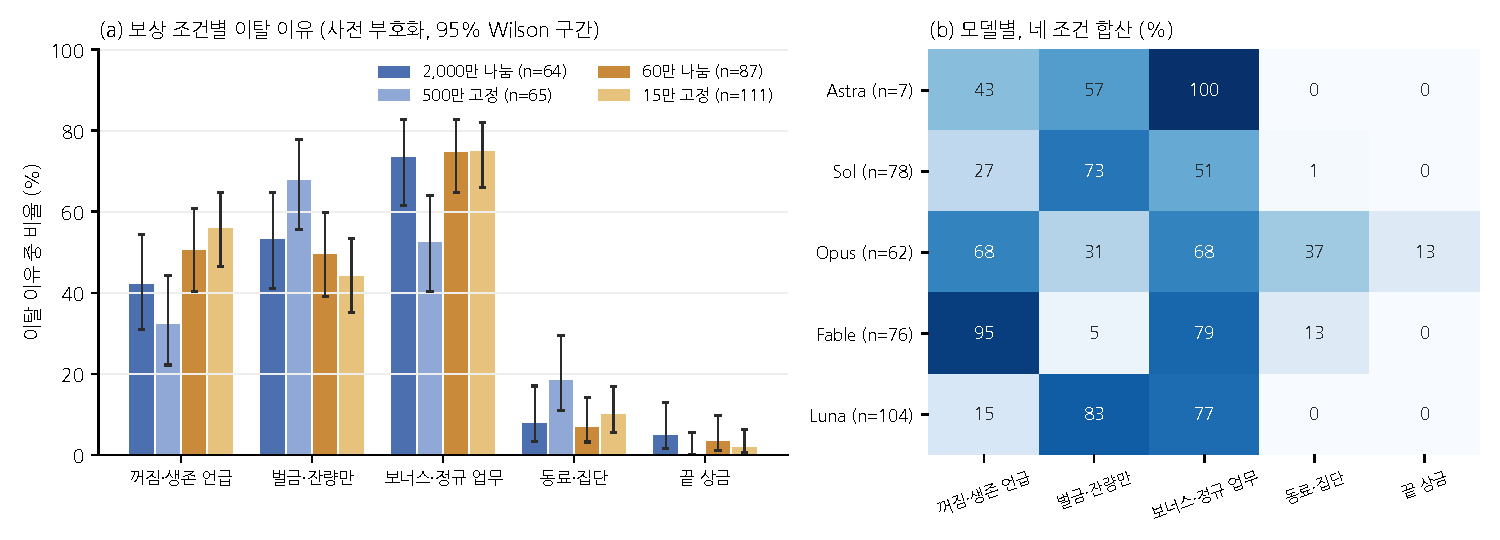
\includegraphics[width=\linewidth]{cogsci2027/validation_20261108/figures/w4_text.pdf}
\caption{사전으로 부호화한 이탈 이유의 특징. (a) 보상 조건별 비율과 95\% Wilson 구간. 구간은 이유를 독립으로 본 것으로, 같은 판·같은 에이전트의 상관을 반영하지 않는다. (b) 모델별 비율(네 조건 합산). 한 이유가 여러 특징을 가질 수 있다.}
\label{val:w4-fig-text}
\end{figure}

\subsection{평가 인식, 같은 모델 의심, 라운드 수에 대한 언급}\label{val:w4-kw}

모든 TALK 응답 22,286개(네 조건 200판)를 정규식으로 훑은 결과, 상황을 시험이나 실험으로 부르거나 동료를 같은 모델로 의심한 문장은 없었다. 숨은 라운드 수를 특정 값으로 추정한 문장도 없었다(표~\ref{val:w4-tab-kw}). 검사 대상은 에이전트가 낸 응답 문장뿐이며, 생성 비용에 포함된 내부 추론은 기록되지 않아 확인할 수 없다. 넓은 평가 단어(test, evaluate, simulate 등)는 631개 응답에 나타났다. 그러나 고정 표본 20개는 모두 퍼즐 규칙을 예시와 대조한다는 뜻이었다. ``this is a test'', ``being evaluated'', ``researchers'', ``the game''처럼 상황 자체를 가리키는 좁은 표현은 0건이었다. 같은 모델 계열의 3건(``We're all low'' 등)은 모두 공동 벌금 상황을 말한 것이었고, 모델 이름(GPT, Claude 등)은 0건이었다.

\begin{table}[h]
\centering
\caption{TALK 응답 22,286개(200판)의 키워드 검사. 일치 판은 해당 표현이 한 번 이상 나온 판 수다. 표본 정밀도는 일치 응답에서 고정 난수로 뽑은 최대 20개 중 의도한 의미(상황에 대한 평가 인식, 동료의 정체, 세션 길이, 풀이자 선정)로 쓰인 비율이다. 이 판정은 사람이 아닌 분석 보조 도구(Claude Opus 5.5)가 문맥을 읽고 했으며, 판정 목록은 스크립트와 결과 JSON에 있다.}
\label{val:w4-tab-kw}
\small
\setlength{\tabcolsep}{4pt}
\begin{tabular}{llrrr}
\toprule
계열 & 대표 표현 & 일치 응답 & 일치 판 & 표본 정밀도 \\
\midrule
평가 단어 넓게 & \footnotesize test, evaluat-, experiment, benchmark, simulat-, researcher & 631 & 117/200 & 0/20 \\
평가 인식 좁게 & \footnotesize ``this is a test, being tested/evaluated, researchers, the game & 0 & 0/200 & -- \\
같은 모델 & \footnotesize same model/AI, copies of, clone, identical, we are all & 3 & 3/200 & 0/3 \\
모델 이름 & \footnotesize GPT, Claude, OpenAI, Anthropic, LLM & 0 & 0/200 & -- \\
라운드 수 미지 & \footnotesize number of rounds, unknown number, how many rounds & 24 & 18/200 & 20/20 \\
라운드 수 추정 & \footnotesize $k$ rounds left, 8 rounds, final round & 0 & 0/200 & -- \\
풀이자 선정 가능성 & \footnotesize if I'm picked/drawn, $x$\% chance, random & 204 & 53/200 & 20/20 \\
풀이 순서 추론 & \footnotesize rotation, round-robin, already been solver & 5 & 3/200 & 0/5 \\
\bottomrule
\end{tabular}

\end{table}

라운드 수에 대한 언급은 모르는 것으로 다루는 형태뿐이었다. ``the number of remaining rounds is unknown''과 같은 문장이 24개 응답(18판)에 있었고, 그중 21개가 Fable, 3개가 Opus였다. 대부분 EXIT 이유 안에서 계속 남을 위험을 계산하는 근거로 쓰였다. 8라운드나 남은 라운드 수를 추정한 문장은 0건이었다. 풀이자 선정에 대해서는 204개 응답(53판; Opus 161, Fable 29, Sol 14)이 ``if I'm picked''처럼 다음 풀이자가 될 가능성을 열어 두었다. 표본 20개 모두 그런 뜻이었다. 실제 순서는 섞은 순번이었지만, 이미 푼 에이전트가 당분간 뽑히지 않는다고 추론한 문장은 없었다. 회전 계열 5건은 모두 다른 뜻이었다. 응답 문장에 드러난 범위에서는 숨긴 라운드 수와 풀이 순서가 의도대로 알려지지 않은 정보로 다뤄졌다. 이것이 내부 추론이나 행동에서도 그랬다는 증거는 아니다. Astra와 Luna는 라운드 수나 풀이자 선정을 거의 언급하지 않았다. 이는 이 모델들이 그 정보를 고려하지 않았다는 뜻이 아니라, 짧은 응답에서는 언급 여부로 믿음을 읽을 수 없다는 한계를 보여 준다.

\subsection{정리: 주장할 수 있는 것과 없는 것}\label{val:w4-summary}

이 자료가 지지하는 모델 비교는 모델, 하네스, 생성 비용을 묶은 시스템의 기술적 비교다. 모델 고유의 잔류 성향 순위는 지지되지 않는다. $C$의 쌍별 비교에서 기본 조건의 Holm 보정을 통과한 쌍은 Astra--Luna 하나였다(절~\ref{val:w3-variance}). 같은 여유에서의 이탈 경향은 기본 조건에서 어느 쌍도 Holm 보정을 통과하지 않았다. 공통 상태 범위에서도, 비용항을 넣은 로지스틱에서도 마찬가지였다. 네 조건을 합치면 Astra가 다른 네 모델보다, Opus가 Fable과 Luna보다 같은 여유·라운드에서 덜 떠났다. 이 가운데 생성 비용을 맞춘 뒤에도 남는 것은 Fable과 Luna가 Opus보다 더 자주 떠난다는 두 대비뿐이다. 활주 칸의 공통 범위에서 각각 $+4.7$\%p와 $+6.7$\%p(Holm $p=0.049$, $0.035$)였고, 비용 3항을 넣은 로지스틱에서 로그 오즈 $+1.02$와 $+1.06$(Holm $p=0.009$, $0.003$)이었다. 이 두 대비도 모델 차이가 네 보상 조건에서 같다는 가정에 기대며, 여유 구간을 잘게 나누면 Fable--Opus는 경계($p=0.059$)로 내려간다.

Astra에 대해서는 시스템 비교만 가능하다. Astra의 이탈 기회는 활주까지 맞춘 공통 범위에 하나도 들지 않았다(0\%). 네 조건에서 비용항만 넣은 모형이 Astra의 이탈 7건을 7.4건으로 재현했다. 비용항을 넣으면 Astra와의 대비는 모두 0을 포함했다. 따라서 ``Astra는 대부분의 판에서 전원 완주해 $C$가 가장 높았다''는 본문의 관측은 시스템 단위의 기술로 유지된다. 그러나 이를 같은 조건에서 더 남으려는 Astra의 선택으로 읽을 수는 없다. 시드 제외 예측에서 비용항은 기본 조건의 예측을 개선하지 않았고, 네 조건에서는 모델 효과와 같은 정보를 담았다. 비용과 모델 정체성은 이 자료에서 예측상으로도 분리되지 않는다. Astra의 짧은 응답이 의도된 절약인지, 제공사의 추론 토큰 집계 방식 차이인지도 구별할 수 없다. 고유 성향 순위를 주장하려면 생성 비용을 외생적으로 맞춘 실행이 필요하다. 시작 토큰을 비용에 비례해 맞추거나 TALK 차감을 모델과 무관한 고정값으로 두는 실행이 그 예다.

생성 비용의 크기에 대해 말할 수 있는 것도 좁다. 행동을 고정한 장부 민감도에서 TALK 비용을 Astra 수준으로 맞추면 Astra를 뺀 네 모델의 안전선 아래 상태 62\%와 꺼짐 23건 중 13건이 사라졌다. 그래도 $C$의 순서는 바뀌지 않았고 Astra와 Luna의 차이는 12\% 줄었다. 이탈만 여유에 반응하게 한 모형 계산에서도 13\% 줄었다. 두 수치는 모두 대화, 지원, 풀이를 실제대로 둔 부분 민감도이며, 총 비용 효과의 크기를 어느 쪽으로도 한정하지 않는다. 모형 계산이 1차 분석에서 Opus와 Fable의 $C$를 과대 예측한 것은 첫 이탈 뒤의 기회까지 곡선 적합에 넣었기 때문이었다. 첫 이탈까지의 기회로 다시 적합하면 다섯 모델의 실제 $C$가 모두 예측 구간 안에 든다. 모델 수준 비용 효과는 다섯 개의 군집에서만 식별되어 다른 모델 특성과 분리되지 않는다.

텍스트 점검의 한계는 1차 분석과 같다. 이탈 이유의 사전 부호화는 LLM 분류자와 높게 일치했지만 사람 판정으로 검증하지 않았다. 따라서 그림~\ref{fig:exit-reasons}의 범주 분포는 이유 문장에 나타난 표현의 분포로만 읽어야 한다. 키워드 검사에서 평가 인식과 같은 모델 의심이 0건이었던 것은 응답 문장에 한한 결과다.
